\chapter{Gradientenverfahren}
Zur Optimierung des neuronalen Netzes wird ein Gradientenverfahren eingesetzt \imgref{gradient}. Ziel dieses Verfahrens ist es ein Minimum zu finden. Dabei wird die Steigung an der aktuellen Position berechnet und anhand des Vorzeichens entschieden ob sich die nächste Position rechts oder links von der aktuellen Stelle befinden soll. Bei einem negativen Vorzeichen ist die Richtung rechts, bei einem positiven links. Dieser Vorgang wird solange wiederholt, bis die Steigung in einem Punkt den Wert \emph{0}, oder ein bestimmten Wert vorgegebenen Wert erreicht.

\begin{figure}[h!]
	\begin{center}
	\fbox{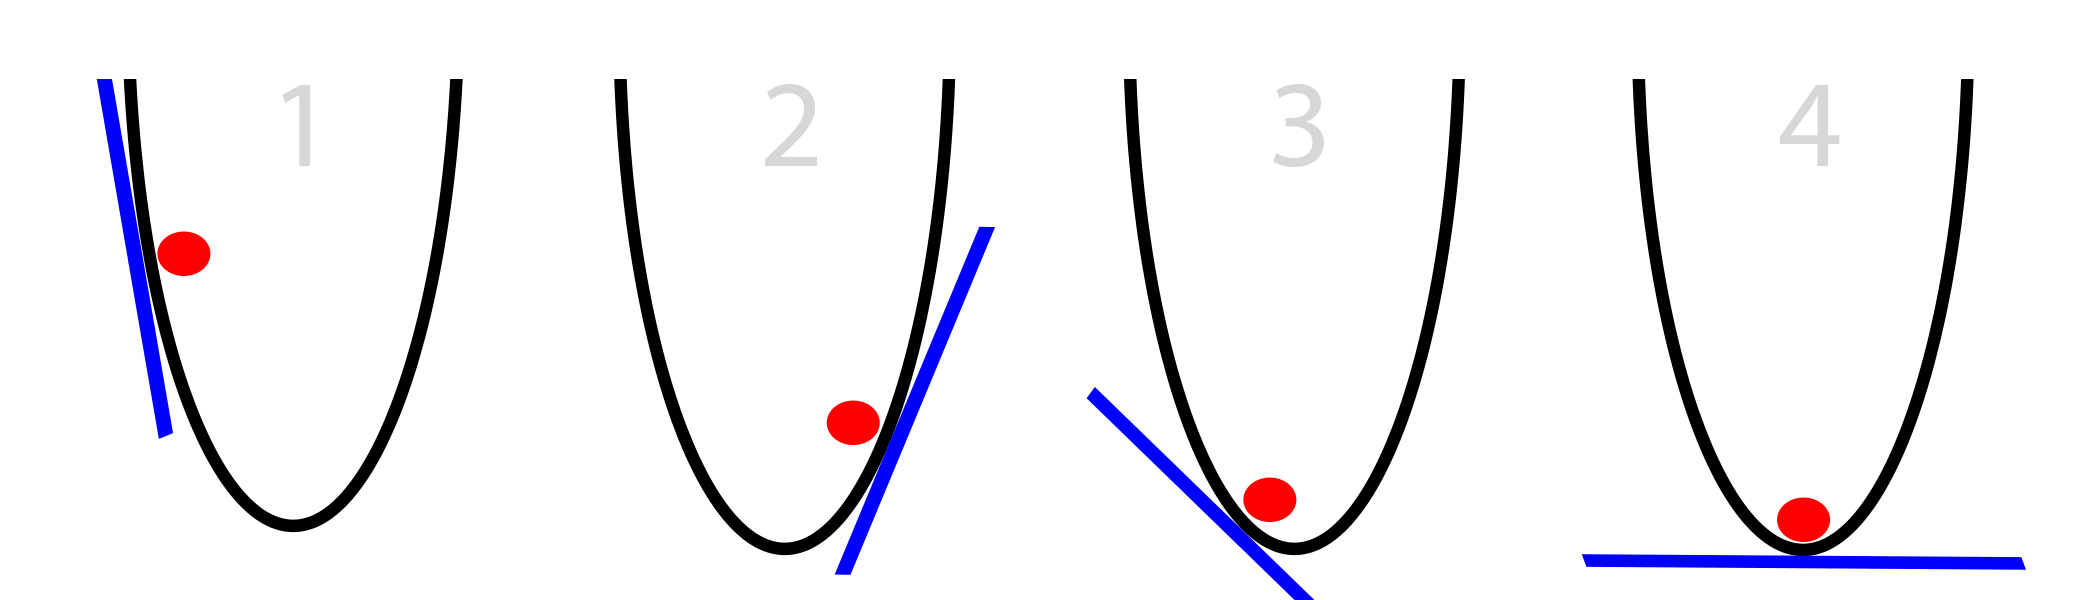
\includegraphics[width=0.9\textwidth]{pictures/sgd_optimal.png}}
	\caption{Gradientenverfahren}
	\label{gradient}
	\end{center}
\end{figure}

Die Schwierigkeit besteht darin, einen geeigneten Faktor zu bestimmen um den die Position geändert wird. Ein einfacher Ansatz ist es dabei die Verschiebung anhand der Steigung zu bestimmen. Je größer der Wert einer positiven Steigung, umso weiter wird die Position nach links verschoben, je kleiner der Wert umso geringer fällt die Richtungsänderung aus. Je weiter man sich dem Minimum nähert, umso geringer fallen die Änderungen aus. Sollte der Nullpunkt erreicht werden, konvergiert das Verfahren. Bei zu großen Richtungsänderungen kann das Verfahren divergieren und man entfernt sich immer weiter von dem gesuchten Minimum.

Um dies zu verhindern wird ein \emph{alpha} Wert eingeführt. Der Wertebereich von \emph{alpha} liegt zwischen 0 und 1. Die neue Position wird nun durch den alten Positionswert und dem Produkt aus Steigung und Alphawert ermittelt. Bei der Wahl eines geeigneten Alpha Wertes muss berücksichtigt werden, dass ein zu kleiner Wert das Gradientenverfahren ausbremst und ein zu großer Wert den Einfluss auf das Ergebniss minimiert.
\todo[inline]{formel?}

\begin{figure}[h!]
	\begin{center}
	\fbox{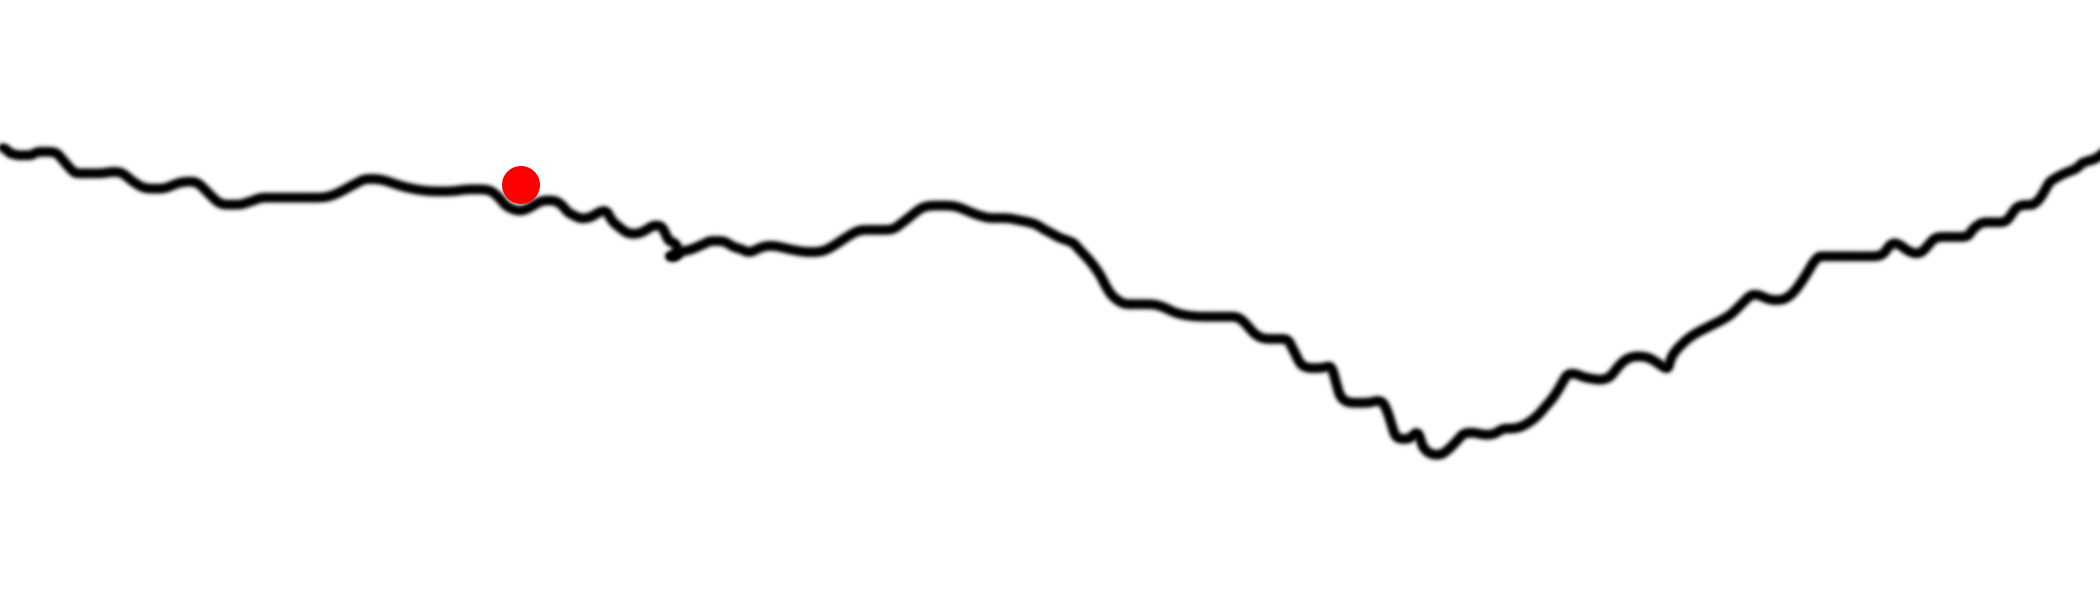
\includegraphics[width=0.7\textwidth]{pictures/alpha_small1.png}}
	\caption{Alpha-Wert Einfluss (Teil 1)}
	\label{alpha1}
	\end{center}
\end{figure}

Die Wahl eines zu geringen Alpha-Wertes führt zu zwei Problemen. Zum einen kann das Verfahren sich in lokalen Minima festsetzen \imgref{alpha1}, sodass das eigentliche Minimum des zu untersuchenden Abschnittes nicht gefunden wird. Im zweiten Fall \imgref{alpha2} fallen die Änderungen bedingt durch ein zu geringes Alpha so gering aus, dass sich die Laufzeit zum auffinden des Minimums enorm steigert.

\begin{figure}[h!]
	\begin{center}
	\fbox{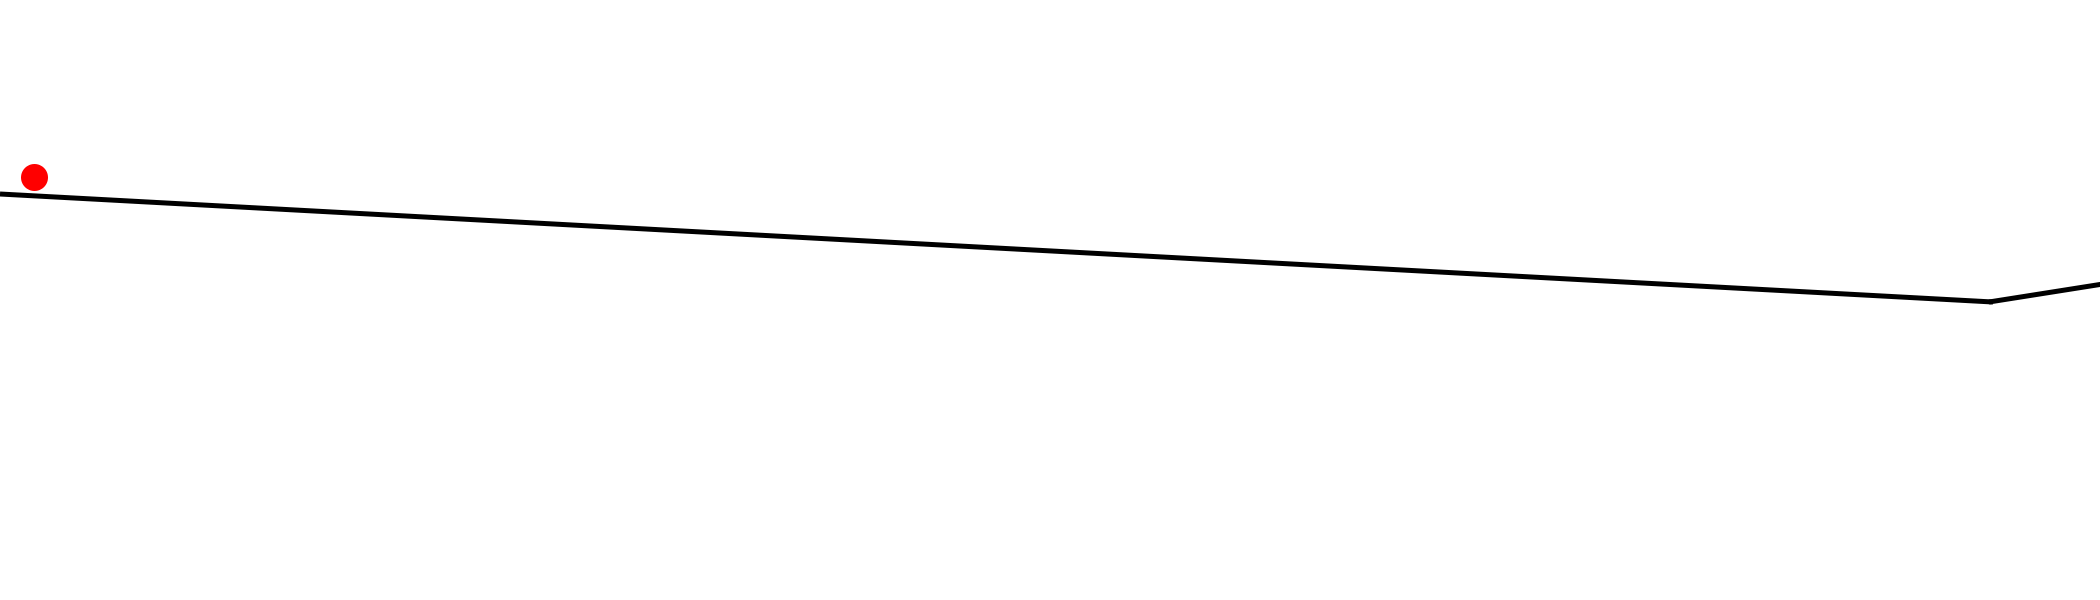
\includegraphics[width=0.7\textwidth]{pictures/alpha_small2.png}}
	\caption{Alpha-Wert Einfluss (Teil 2)}
	\label{alpha2}
	\end{center}
\end{figure}